\documentclass[12pt,letterpaper]{exam}
\usepackage[lmargin=1in,rmargin=1in,tmargin=1in,bmargin=1in]{geometry}
\usepackage{../style/exams}

% -------------------
% Course & Exam Information
% -------------------
\newcommand{\course}{MAT 101: Exam 3}
\newcommand{\term}{Spring -- 2022}
\newcommand{\examdate}{05/12/2022}
\newcommand{\timelimit}{85 Minutes}

\setbool{hideans}{false} % Student: True; Instructor: False

% -------------------
% Content
% -------------------
\begin{document}

\examtitle
\instructions{Write your name on the appropriate line on the exam cover sheet. This exam contains \numpages\ pages (including this cover page) and \numquestions\ questions. Check that you have every page of the exam. Answer the questions in the spaces provided on the question sheets. Be sure to answer every part of each question and show all your work.} 
\scores
%\bottomline
\newpage

% ---------
% Questions
% ---------
\begin{questions}

% Question 1
\newpage
\question Compute the functions at the indicated value below. Your answers should be exact. \pspace

\begin{parts}
\part[2] $f(x)= -4(5^x)$ \vfill
	\[
	f(2)= -4(5^2)= -4(25)= -100 \hspace{4.3cm}
	\] \vfill

\part[2] $g(x)= 5(2^x)$ \vfill
	\[
	g(0)= 5(2^0)= 5(1)= 5 \hspace{5.9cm}
	\] \vfill

\part[2] $h(x)= -6(4^{1 - 2x})$ \vfill
	\[
	h(1)= -6(4^{1 - 2(1)})= -6(4^{1 - 2})= -6(4^{-1})= -6 \cdot \dfrac{1}{4}= -\dfrac{3}{2}
	\] \vfill

\part[2] $r(x)= 7 \left( \dfrac{3}{5} \right)^x$ \vfill
	\[
	r(-2)= 7 \left( \dfrac{3}{5} \right)^{-2}= 7 \left( \dfrac{5}{3} \right)^2= 7 \cdot \dfrac{25}{9}= \dfrac{175}{9} \hspace{2.4cm}
	\] \vfill

\part[2] $s(x)= 8(9^x)$ \vfill
	\[
	s \left( -\frac{1}{2} \right)= 8(9^{-1/2})= 8 \cdot \dfrac{1}{9^{1/2}}= 8 \cdot \dfrac{1}{\sqrt{9}}= 8 \cdot \dfrac{1}{3}= \dfrac{8}{3} \hspace{1.2cm}
	\]
\end{parts}



% Question 2
\newpage
\question Using exact values, write the following functions in the form $y= Ab^x$: \pspace

\begin{parts}
\part[3] $f(x)= -5(3^{2x})$ \pvspace{2.5cm}

	\[
	f(x)= -5 \big( (3^2)^x \big)= -5(9^x)
	\] \pvspace{2.5cm}

\part[3] $g(x)= 3 \left( \dfrac{5}{7} \right)^{-x}$ \pvspace{2.35cm}
	\[
	g(x)= 3 \left( \dfrac{5}{7} \right)^{-x}= 3 \left( \left( \dfrac{5}{7} \right)^{-1} \right)^x= 3 \left( \dfrac{7}{5} \right)^x
	\] \pvspace{2.35cm}

\part[4] $h(x)= 5 (2^{1 - 3x})$ \pvspace{2.5cm}
	\[
	h(x)= 5 (2^{1 - 3x})= 5(2^1 \cdot 2^{-3x})= 10(2^{-3x}) 10 \big( (2^{-3})^x \big)= 10 \left( \dfrac{1}{2^3} \right)^x= 10 \left( \dfrac{1}{8} \right)^x
	\]
\end{parts}



% Question 3
\newpage
\question Determine whether the following functions are increasing or decreasing: \pspace

\begin{parts}
\part[3] $f(x)= 3 \left( \dfrac{10}{11} \right)^x$ \pvspace{2.55cm}

{\itshape Because $f(x)$ is an exponential function of the form $y= Ab^{cx}$ with $b= \frac{10}{11} < 1$, $c= 1 > 0$, and $A= 3 > 0$, $f(x)$ is a decreasing function.} \pvspace{2.55cm}

\part[3] $g(x)= 17 (5^{-2x})$ \pvspace{2.6cm}

{\itshape Because $g(x)$ is an exponential function of the form $y= Ab^{cx}$ with $b= 5 > 1$, $c= -2 < 0$, and $A= 17 > 0$, $f(x)$ is a decreasing function.} \pvspace{2.6cm}

\part[4] $h(x)= -9 \left( \dfrac{7}{5} \right)^{2 - x}$ \pvspace{2.6cm}

{\itshape We have\dots
	\[
	h(x)= -9 \left( \dfrac{7}{5} \right)^{2 - x}= -9 \left( \dfrac{7}{5} \right)^2 \left( \dfrac{7}{5} \right)^{-x}= -9 \left( \dfrac{49}{25} \right) \left( \dfrac{7}{5} \right)^{-x}= -\dfrac{441}{25} \left( \dfrac{7}{5} \right)^{-x}
	\]
Because $h(x)$ is an exponential function of the form $y= Ab^{cx}$ with $b= \frac{7}{5} > 1$, $c= -1 < 0$, and $A= -\frac{441}{25} < 0$, $f(x)$ is an increasing function.
} 
\end{parts}



% Question 4
\newpage
\question[10] Sketch the function $y= -2 \left( \dfrac{1}{3} \right)^{x - 1}$ on the graph below. 
	\[
	\fbox{
	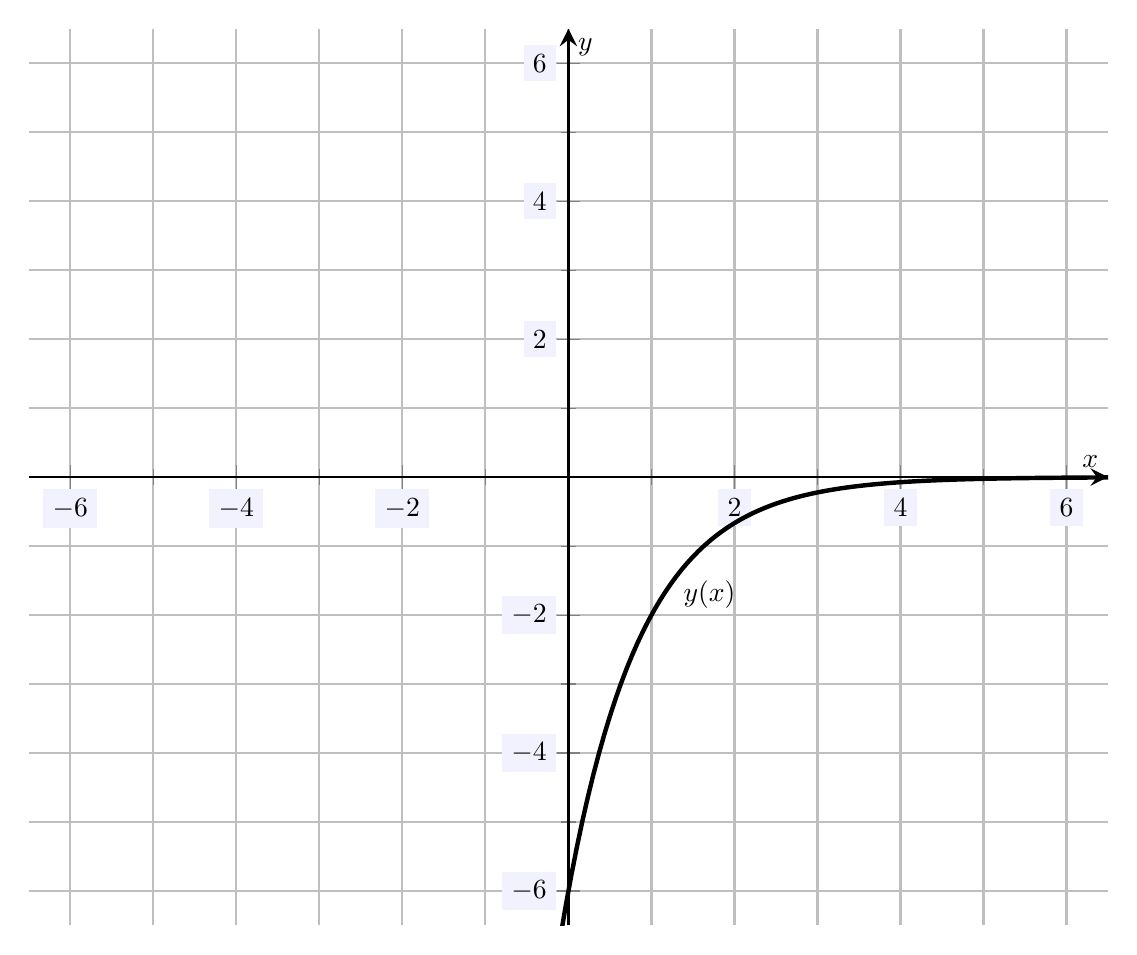
\begin{tikzpicture}[scale=2,every node/.style={scale=0.5}]
	\begin{axis}[
	grid=both,
	axis lines=middle,
	ticklabel style={fill=blue!5!white},
	xmin= -6.5, xmax=6.5,
	ymin= -6.5, ymax=6.5,
	xtick={-6,-4,-2,0,2,4,6},
	ytick={-6,-4,-2,0,2,4,6},
	minor tick = {-7,-6,...,7},
	xlabel=\(x\),ylabel=\(y\),
	]
	\node at (1.7,-1.7) {$y(x)$};
	\addplot[thick, domain= -0.1:6.5, samples=100] ({x},{-2*(1/3)^(x -1)});
	\end{axis}
	\end{tikzpicture}
	}
	\]

	\[
	\begin{aligned}
	y&= -2 \left( \dfrac{1}{3} \right)^{x - 1}= -2 \left( \dfrac{1}{3} \right)^{-1} \left( \dfrac{1}{3} \right)^x= -2 \cdot 3 \left( \dfrac{1}{3} \right)^x= -6 \left( \dfrac{1}{3} \right)^x \\[0.3cm]
	y(0)&= -6 \left( \dfrac{1}{3} \right)^0= -6 \cdot 1= -6
	\end{aligned}
	\]

{\itshape Because $y$ is an exponential function of the form $y= Ab^{cx}$ with $b= \frac{1}{3} < 1$, $c= 1 > 0$, and $A= -6 < 0$, $f(x)$ is an increasing function. By the work above, we know the $y$-intercept is $-6$, i.e. $(0, -6)$. Using these two facts about $y$, we are able to give the sketch above.} 



% Question 5
\newpage
\question[10] Find the exact values of the following: \pspace

\begin{enumerate}[(a)]
\item $\log_3 3^{2022}= 2022$ \vfill

\item $\log_6 \left( \dfrac{1}{6^{1995}} \right)= \log_6(6^{-1995})= -1995$ \vfill

\item $\log_7 1= 0$ \vfill

\item $\ln(e^{10/11})= \dfrac{10}{11}$ \vfill

\item $\log_2(64)= \log_2(2^6)= 6$ \vfill
\end{enumerate}



% Question 6
\newpage
\question[10] Write the following as a single logarithm involving no negative powers:
	\[
	5 \log_3(x) - 2 \log_3(y) - 6 \log_3(z^{-1}) + 4
	\] \pvspace{1.5cm}
	
	\[
	\begin{aligned}
	5 \log_3(x) - 2 \log_3(y) - 5 \log_3(z^{-1}) + 4&= 5 \log_3(x) - 2 \log_3(y) - 5 \log_3(z^{-1}) + \log_3(3^4) \\[0.5cm]
	&= 5 \log_3(x) - 2 \log_3(y) - 6 \log_3(z^{-1}) + \log_3(81) \\[0.5cm]
	&= \log_3(x^5) + \log_3(y^{-2}) + \log_3(z^6) + \log_3(81) \\[0.5cm]
	&= \log_3(81 x^5 y^{-2} z^6) \\[0.5cm]
	&= \log_3 \left( \dfrac{81x^5 z^6}{y^2} \right)
	\end{aligned}
	\]



% Question 7
\newpage
\question[10] Write the following in terms of $\ln x$, $\ln y$, and $\ln z$:
	\[
	\ln \left( \dfrac{x^{10}}{y^{-5} z^7} \right)
	\] \pvspace{1.5cm}
	
	\[
	\begin{aligned}
	\ln \left( \dfrac{x^{10}}{y^{-5} z^7} \right)&= \ln(x^{10}) - \ln(y^{-5} z^7) \\[0.5cm]
	&=  \ln(x^{10}) - \bigg( \ln(y^{-5}) + \ln(z^7) \bigg) \\[0.5cm]
	&=  10 \ln(x) - \bigg( -5 \ln(y) + 7\ln(z) \bigg) \\[0.5cm]
	&=  10 \ln(x) + 5 \ln(y) - 7\ln(z)
	\end{aligned}
	\]



% Question 8
\newpage
\question[10] Use the change of base formula to convert $\log_8(4)$ to base-2 and then find the exact value. \pvspace{1.5cm}
	
	\[
	\begin{aligned}
	log_8(4)&= \dfrac{\log_2(4)}{\log_2(8)} \\[0.5cm]
	&= \dfrac{\log_2(2^2)}{\log_2(2^3)} \\[0.5cm]
	&= \dfrac{2}{3}
	\end{aligned}
	\]



% Question 9
\newpage
\question Complete the following:

\begin{parts}
\part[5] How many digits does $2021^{2022}$ have in base-10? \pvspace{1.5cm}

	\[
	\log_{10}(2021^{2022})= 2022 \log_{10}(2021) \approx 2022(3.30557) \approx 6683.86
	\] \pvspace{1cm}

{\itshape Therefore, $2021^{2022}$ has 6,684 digits in base-10.} \pvspace{6cm}

\part[5] How many digits does $2021^{2022}$ have in base-8? \pvspace{1.5cm}

	\[
	\log_8(2021^{2022})= 2022 \log_8(2021) \approx 2022(3.66028) \approx 7401.09
	\] \pvspace{1cm}

{\itshape Therefore, $2021^{2022}$ has 7,402 digits in base-8.}
\end{parts}



% Question 10
\newpage
\question[10] Is there a whole number $k$ such that $2022^k$ has 15,000 digits? Explain. \pvspace{1.5cm}

{\itshape The number of digits in $2022^k$ is the smallest whole number that is strictly larger than $\log_{10}(2022^k)$. If we want this to be 15,000, then we need\dots \pspace
	\[
	\begin{aligned}
	14999 &\leq \log_{10}(2022^k) < 15000 \\[0.5cm]
	14999 &\leq k \log_{10}(2022) < 15000 \\[0.5cm]
	\dfrac{14999}{\log_{10}(2022)} &\leq \dfrac{k \log_{10}(2022)}{\log_{10}(2022)} < \dfrac{15000}{\log_{10}(2022)} \\[0.5cm]
	\end{aligned}
	\]
	\[
	\dfrac{14999}{3.305781151} \leq  k < \dfrac{15000}{3.305781151}
	\] \par
	\[
	4537.2 \leq k < 4537.51
	\] \pspace
However, there is no whole number between $4537.2$ and $4537.51$. Therefore, there is no whole number $k$ such that $2022^k$ has 15,000 digits.}



% Question 11
\newpage
\question[10] Showing all your work, find the exact solution to the following: 
	\[
	\dfrac{1}{25^x} - 4= 1
	\] \pvspace{1.3cm}
	
{\itshape There are many approaches. For instance, \pspace
	\[
	\begin{aligned}
	\dfrac{1}{25^x} - 4&= 1 \\[0.5cm]
	\dfrac{1}{25^x}&= 5 \\[0.5cm]
	25^{-x}&= 5 \\[0.5cm]
	(5^2)^{-x}&= 5 \\[0.5cm]
	5^{-2x}&= 5 \\[0.5cm]
	-2x&= 1 \\[0.5cm]
	x&= -\dfrac{1}{2}
	\end{aligned}
	\] \pspace
	
	\begin{center} {\bfseries OR} \end{center}
	
	\[
	\begin{aligned}
	\dfrac{1}{25^x} - 4&= 1 \\[0.5cm]
	\dfrac{1}{25^x}&= 5 \\[0.5cm]
	25^{-x}&= 5 \\[0.5cm]
	\log_{25}(25^{-x})&= \log_{25}(5) \\[0.5cm]
	-x&= \dfrac{1}{2} \\[0.5cm]
	x&= -\dfrac{1}{2}
	\end{aligned}
	\] 
}



% Question 12
\newpage
\question[10] Showing all your work, find the exact solution to the following:  
	\[
	15 - \log_2(4 - x)= 10
	\] \pvspace{1.3cm}

	\[
	\begin{aligned}
	15 - \log_2(4 - x)&= 10 \\[0.5cm]
	\log_2(4 - x)&= 5 \\[0.5cm]
	2^{\log_2(4 - x)}&= 2^5 \\[0.5cm]
	4 - x&= 32 \\[0.5cm]
	x&= -28
	\end{aligned}
	\]



% Question 13
\newpage
\question[10] Showing all your work, find the exact solution to the following: 
	\[
	e^{x/3} + 12= 20
	\] \pvspace{1.3cm}

	\[
	\begin{aligned}
	e^{x/3} + 12&= 20 \\[0.5cm]
	e^{x/3}&= 8 \\[0.5cm]
	\ln(e^{x/3})&= \ln(8) \\[0.5cm]
	\dfrac{x}{3}&= \ln(8) \\[0.5cm]
	x&= 3 \ln(8)
	\end{aligned}
	\]



% Question 14
\newpage
\question[10] Showing all your work, find the exact solution to the following: 
	\[
	\ln(3x) + 10= 8
	\] \pvspace{1.3cm}

	\[
	\begin{aligned}
	\ln(3x) + 10&= 8 \\[0.5cm]
	\ln(3x)&= -2 \\[0.5cm]
	e^{\ln(3x)}&= e^{-2} \\[0.5cm]
	3x&= e^{-2} \\[0.5cm]
	x&= \dfrac{e^{-2}}{3} \\[0.5cm]
	x&= \dfrac{1}{3e^2}
	\end{aligned}
	\]



% Question 15
\newpage
\question[10] Showing all your work, find the exact solution to the following: 
	\[
	3\left( \dfrac{1}{2} \right)^{5x + 3}= 45
	\] \pvspace{0.2cm}

{\itshape There are many approaches. For instance, \pvspace{0.1cm}
	\[
	\begin{aligned}
	3\left( \dfrac{1}{2} \right)^{5x + 3}&= 45 \\[0.25cm]
	\left( \dfrac{1}{2} \right)^{5x + 3}&= 15 \\[0.25cm]
	\ln\left( \dfrac{1}{2} \right)^{5x + 3}&= \ln(15) \\[0.25cm]
	(5x + 3) \ln\left( \dfrac{1}{2} \right)&= \ln(15) \\[0.25cm]
	5x + 3&= \dfrac{\ln(15)}{\ln(1/2)} \\[0.25cm]
	5x&= \dfrac{\ln(15)}{\ln(1/2)} - 3 \\[0.25cm]
	x&= \dfrac{\dfrac{\ln(15)}{\ln(1/2)} - 3}{5}
	\end{aligned}
	\] \pvspace{0.2cm}

\begin{center} {\bfseries OR} \end{center}

	\[
	\begin{aligned}
	3\left( \dfrac{1}{2} \right)^{5x + 3}&= 45 \\[0.25cm]
	\left( \dfrac{1}{2} \right)^{5x + 3}&= 15 \\[0.25cm]
	\log_{1/2} \left( \dfrac{1}{2} \right)^{5x + 3}&= \log_{1/2}(15) \\[0.25cm]
	5x + 3&= \log_{1/2}(15) \\[0.25cm]
	5x&= \log_{1/2}(15) - 3 \\[0.25cm]
	x&= \dfrac{\log_{1/2}(15) - 3}{5}
	\end{aligned}
	\]
}



% Question 16
\newpage
\question[10] Showing all your work, find the exact solution to the following: 
	\[
	3 - \log_2(x)= \log_2(x + 2)
	\] \pvspace{1.5cm}
	
{\itshape Observe that we have\dots
	\[
	\begin{aligned}
	3 - \log_2(x)&= \log_2(x + 2) \\[0.5cm]
	\log_2(x + 2) + \log_2(x)&= 3 \\[0.5cm]
	\log_2\big( (x + 2)x \big)&= 3 \\[0.5cm]
	\log_2(x^2 + 2x)&= 3 \\[0.5cm]
	2^{\log_2(x^2 + 2x)}&= 2^3 \\[0.5cm] 
	x^2 + 2x&= 8 \\[0.5cm]
	x^2 + 2x - 8&= 0 \\[0.5cm]
	(x + 4)(x - 2)&= 0
	\end{aligned}
	\] \pspace
But then either $x + 4= 0$, i.e. $x= -4$, or $x - 2= 0$, i.e. $x= 2$. However, if $x= -4$, then the original equality would be $3 - \log_2(-4)= \log_2(-2)$ and $\log_2 x$ is only defined for $x > 0$. Therefore, the only solution is $x= 2$.}



% Question 17
\newpage
\question[10] Suppose Alice invests \$5,000 into an account which earns 4.5\% annual interest, compounded monthly. How much will the investment be worth in 8~years? How much interest has been earned during this time period? \pvspace{1.5cm}

{\itshape For discrete compounded interest, we know that $F= P \left(1 + \dfrac{r}{k} \right)^{kt}$, where $F$ is the future value, $P$ is the present value, $r$ is the annual interest rate, $k$ is the number of compounds per year, and $t$ is the number of years. But then we have\dots \pspace
	\[
	\begin{aligned}
	F&= P \left(1 + \dfrac{r}{k} \right)^{kt} \\[0.5cm]
	F&= 5000 \left(1 + \dfrac{0.045}{12} \right)^{12 \cdot 8} \\[0.5cm]
	F&= 5000 (1.00375)^{96} \\[0.5cm]
	F&\approx 5000(1.432364654) \\[0.5cm]
	F&\approx \$7161.82
	\end{aligned}
	\] \pspace
Because only \$5,000 was invested, the interest earned must be $\$7161.82 - \$5000= \$2161.82$. 
}



% Question 18
\newpage
\question[10] Bob takes out a \$750 loan with an interest rate of 6.4\%, compounded continuously. Supposing the loan ends after two and a half years, how much does Bob owe after this time? How much total interest does he pay on this loan? \pvspace{1.5cm}

{\itshape For continuous compounded interest, we know that $F= P e^{rt}$, where $F$ is the future value, $P$ is the present value, $r$ is the annual interest rate, and $t$ is the number of years. But then we have\dots \pspace
	\[
	\begin{aligned}
	F&= P e^{rt} \\[0.5cm]
	F&= 750 e^{0.064 \cdot 2.5} \\[0.5cm]
	F&\approx 750 (1.173511) \\[0.5cm]
	F&\approx \$880.13
	\end{aligned}
	\] \pspace
Because only \$750 was taken out on the loan, the interest must be $\$880.13 - \$750= \$130.13$.
}



% Question 19
\newpage
\question[10] Suppose Montez takes out a loan to expand his small business. The loan is for \$25,000 at a 3.8\% annual interest rate, compounded quarterly. How long until the amount of money he owes on the loan has doubled? \pvspace{1.5cm}

{\itshape For discrete compounded interest, we know that $F= P \left(1 + \dfrac{r}{k} \right)^{kt}$, where $F$ is the future value, $P$ is the present value, $r$ is the annual interest rate, $k$ is the number of compounds per year, and $t$ is the number of years. But then we have\dots \pspace
	\[
	\begin{aligned}
	F&= P \left(1 + \dfrac{r}{k} \right)^{kt} \\[0.5cm]
	50000&= 25000 \left(1 + \dfrac{0.038}{4} \right)^{4t} \\[0.5cm]
	50000&= 25000 (1.0095)^{4t} \\[0.5cm]
	(1.0095)^{4t}&= 2 \\[0.5cm]
	\ln(1.0095)^{4t}&= \ln(2) \\[0.5cm]
	4t \ln(1.0095)&= \ln(2) \\[0.5cm]
	t&= \dfrac{\ln(2)}{4 \ln(1.0095)} \\[0.5cm]
	t&\approx 18.33 \text{ years}
	\end{aligned}
	\]
}



% Question 20
\newpage
\question[10] Jillian buys \$900 in a stock which promises annual returns of 1.3\%, compounded continuously. How long does Jillian have to wait until this stock is worth \$1,500? \pvspace{1.5cm}

{\itshape For continuous compounded interest, we know that $F= P e^{rt}$, where $F$ is the future value, $P$ is the present value, $r$ is the annual interest rate, and $t$ is the number of years. But then we have\dots \pspace
	\[
	\begin{aligned}
	F&= P e^{rt} \\[0.5cm]
	1500&= 900 e^{0.013t} \\[0.5cm]
	e^{0.013t}&= 1.66667 \\[0.5cm]
	\ln(e^{0.013t})&= \ln(1.66667) \\[0.5cm]
	0.013t&= 0.510828 \\[0.5cm]
	t&\approx 39.29 \text{ years}
	\end{aligned}
	\] \pspace
}


\end{questions}
\end{document}